\documentclass[11pt]{article}
\usepackage[margin=1.05in]{geometry}
\usepackage{amsmath,amssymb,amsthm}
\usepackage{booktabs}
\usepackage{array}
\usepackage{tabularx}
\usepackage[protrusion=true,expansion=false]{microtype}
\usepackage[table]{xcolor}
\usepackage{enumitem}
\usepackage{titlesec}
\usepackage{float}
\usepackage{tikz}
\usetikzlibrary{arrows.meta,positioning,calc,backgrounds}
\usepackage{hyperref}

\hypersetup{colorlinks=true, linkcolor=blue!60!black, urlcolor=blue!60!black, citecolor=blue!60!black}
\usepackage[skip=0.6\baselineskip, indent=0pt]{parskip}

\titleformat{\section}{\large\bfseries}{\thesection.}{0.7em}{}
\titleformat{\subsection}{\normalsize\bfseries}{\thesubsection.}{0.6em}{}

\theoremstyle{plain}
\newtheorem{proposition}{Proposition}
\theoremstyle{definition}
\newtheorem{definition}{Definition}

% ----- notation (as in version 0.4, less BLS) -----
\newcommand{\vmax}{V_{\max}}
\newcommand{\Tc}{T_{\mathrm{close}}}
\newcommand{\bcorr}{b_{\mathrm{corr}}}
\newcommand{\tx}[1]{\texttt{#1}}
\newcommand{\be}[2]{\langle #1\rangle_{#2}}
\newcommand{\pre}[2]{[#1]_{#2}}
\newcommand{\xo}[1]{\mathsf{x}(#1)}
\newcommand{\Ht}[1]{H_{\textsf{#1}}}
\newcommand{\Hb}[1]{H^{340}_{\textsf{#1}}}
\newcommand{\Sign}{\mathsf{Sign}}
\newcommand{\Vfy}{\mathsf{Verify}}
\newcommand{\PSign}{\mathsf{PreSign}}
\newcommand{\PVfy}{\mathsf{PreVerify}}
\newcommand{\Compl}{\mathsf{Complete}}
\newcommand{\Extr}{\mathsf{Extract}}
\newcommand{\Wots}{\mathsf{W}}
\newcommand{\kiss}{k_{\mathrm{iss}}}
\newcommand{\Piss}{P_{\mathrm{iss}}}
\newcommand{\sid}{\mathit{sid}}
\newcommand{\owed}{\mathsf{owed}}
\newcommand{\PH}{P_H^{c}}
\newcommand{\Oc}{O_c}
\newcommand{\KQ}{K_{Q}^{c}}
\newcommand{\Kb}{K_{b}^{c}}
\newcommand{\Kcorr}{K_{\mathrm{corr}}^{c}}
\newcommand{\KU}{K_{U}^{c}}
\newcommand{\Acorr}{A_{\mathrm{corr}}^{c}}
\newcommand{\AU}{A_{U}^{c}}

\newcolumntype{L}{>{\raggedright\arraybackslash}X}
\renewcommand{\arraystretch}{1.3}
\makeatletter
\setlength{\@fptop}{0pt}
\setlength{\@fpsep}{1.5\baselineskip}
\setlength{\@fpbot}{0pt plus 1fil}
\makeatother

\newenvironment{algobox}[1]
  {\par\smallskip\noindent\begin{tabular}{|p{0.955\linewidth}|}\hline\textbf{#1}\\[2pt]}
  {\\\hline\end{tabular}\par\smallskip}

\title{\textbf{The grants L2}\\a Lichen L2 without global order\\[2pt]\large early draft: one note per contract, live receipt}
\author{waxwing}
\date{Version 0.5, November 2026\\[2pt]\small a companion to \emph{Lichen}, version 0.5~\cite{lichen}, and a variant of version 0.4~\cite{grants04}}

\begin{document}
\maketitle

\begin{abstract}
Version 0.4 of the grants L2~\cite{grants04} lets a user hold many notes
and protects at most four of them in an exit. Every limit it then needs
follows from that: claims of up to four notes and fallbacks, a fixed
point over sets to count them, merges that need the hub, aggregate BLS
signatures to keep a claim small, and a hub that can profit from
halting while users hold more notes than a claim can carry.

This version holds the number of notes at one. A payment is a
\emph{joint spend} of the payer's note and the payee's, giving each a
new note; both sign it, and one grant opens both outputs at once. The
payee must therefore be online to be paid, like a Lightning payee. In
return, a claim is one note and at most one spend in flight; Algorithm~1
has three cases; the hub cites at most two spends; there are no merges;
there is nothing for a halting hub to keep; and with one signature per
claim there is nothing to aggregate, so the notes are signed with BIP340
and encrypted by adaptor, and the hub's statement needs no pairing:
about 2.6M cycles (estimated), against 29M. The exit's graph is version
0.4's, with \tx{request}, \tx{correct} and \tx{ack} about 30--45\%
smaller. A deferred receipt through a mailbox is kept as an option, and
set apart (\S\ref{sec:deferred}), so that the live design can be judged
on its own. A proposal; nothing here is built.
\end{abstract}

\tableofcontents

\section{Setting}

The setting is version 0.4's~\cite{grants04}: a Lichen contract
(\cite{lichen}, \S3) locks the hub's liquidity and the user's deposit in
one Bitcoin output, with a cap $\vmax$, reserves $r_A$ and $r_H$, a
close time $\Tc$ and a unit $u$ (sats per unit; an on-chain amount $b$
is a 4-byte word paid out as $u\,b$ sats). It ends by \textbf{fold}
(both sign), \textbf{default} (after $\Tc$: she gets $r_A$) or
\textbf{exit} (she claims $b$; she is paid $b$, or the hub's correction
$\bcorr \le b$ if the hub proves her owed no more). The hub's book is the
only ledger, and nothing is ordered beyond what each spend names.

\textbf{Contracts and credit.} A user's participation is defined by her
contract. Contract $c$ has a fresh L2 key $\Oc$; the note of $\Oc$ is
what $c$'s exit claims. A note under any other key is credit.

\textbf{What is new.} Each contract key holds \emph{exactly one} note at
all times, from the opening (the mint) to the close. Receiving is a
spend of the receiver's note, so the receiver signs it. Everything else
in this paper follows from that rule.

\section{Notation}\label{sec:notation}

As in version 0.4 (\cite{grants04}, \S2), with BLS12-381 removed.

\begin{itemize}[nosep]
\item secp256k1: generator $G$, order $n$; every key x-only
  (BIP340~\cite{bip340}). Lower-case letters scalars, upper-case points.
  $\xo{P}$ the 32-byte x-coordinate; $P^{(33)}$ the point compressed.
\item $\be{v}{k}$: $v$ as $k$ bytes, big-endian. $\pre{h}{k}$: the first
  $k$ bytes of $h$. $\|$: concatenation.
\item $\Ht{tag}(p_1, \dots, p_r)$: the L2's tagged hash, SHA-256 over the
  tag \textsf{lichen/notes/\ldots}, a zero byte, and each part
  length-prefixed. Tags \textsf{note}, \textsf{half}, \textsf{spend},
  \textsf{out}, \textsf{grant-commitment}, \textsf{auth},
  \textsf{unlock}, \textsf{unlock-scalar}, \textsf{issue}.
\item BIP340: $\Sign_d(m)$, $\Vfy_P(m, \sigma)$, 64 bytes. An owner's
  signature on a spend is written $\psi$, the issuer's on a note
  $\sigma$.
\end{itemize}

\textbf{Adaptor signatures}~\cite{poelstra,aumayr} replace version 0.4's
BLS encryption. For a point $T = tG$, the issuer's pre-signature on $m$
is $\rho = \PSign_{\kiss}(m, T) = (R', s')$: it draws $k$ until $R = kG
+ T$ has even $y$, sets $R' = kG$ and $s' = k + e(R, \Piss, m)\,\kiss$.
$\PVfy_{\Piss}(m, T, \rho)$ holds iff $s'G = R' + e(R' + T, \Piss,
m)\Piss$ and $R' + T$ has even $y$. $\Compl(\rho, t) = (\xo{R' + T},\ s'
+ t)$ is an ordinary BIP340 signature on $m$; and $\Extr(\sigma, \rho) =
s - s'$ gives $t$ back. A pre-signature is 65 bytes ($R'$ compressed,
$s'$).

Version 0.4 chose BLS for two reasons: a claim of four notes aggregates
to one signature of 48 bytes, and BLS is unique, so it has no adaptor
(\cite{grants04}, \S2.2) and needed encryption instead. With one note
per claim the first reason is gone, and with BIP340 notes the second
turns around: adaptors are standard, and the statement verifies
BIP340, which RISC Zero accelerates, instead of a pairing. That $\Extr$
recovers $t$ costs nothing here: $t$ always travels in the clear
(\S\ref{sec:payment}).

\textbf{One-time signatures} $\Wots_K(x)$: as in version 0.4. Winternitz,
4-bit digits plus checksum, 2 witness items a digit; SHA-256 chains for
Alice's keys, HASH160 for the hub's; two different signatures under one
key are an \emph{equivocation}.

\textbf{Keys.}
\begin{center}
\begin{tabularx}{\linewidth}{llL}
\toprule
Symbol & Scope & Use \\
\midrule
$\kiss$, $\Piss = \kiss G$ & the deployment & the issuer's key: signs every note; pre-signs every grant's outputs \\
$\PH$, $P_A^c$ & contract $c$ & the 2-of-2 on every link of $c$'s graph \\
$a_c$, $\Oc = a_cG$ & contract $c$ & her L2 key, fresh for $c$: owns $c$'s one note; signs her spends \\
$\KQ$, $\Kb$, $\Acorr$, $\AU$ & contract $c$, hers & one-time: $Q$ and $b$ in \tx{request}; her countersignatures in \tx{ack} \\
$\Kcorr$, $\KU$ & contract $c$, the hub's & one-time: $\bcorr$ and $U$ in \tx{correct} \\
$z_S$, $t_S$, $T_S = t_S G$ & spend $S$ & the unlock: a 16-byte seed, its scalar, its point \\
\bottomrule
\end{tabularx}
\end{center}

\section{Notes, spends and grants}

\subsection{Notes}

\begin{definition}
A \emph{note} is $N = (\mathit{id}, o, v)$: a 32-byte id, an owner, a
value $0 \le v < 2^{48}$ sats. Its short id is $\iota =
\pre{\mathit{id}}{16}$ and its digest $\delta(N) =
\Ht{note}(\pre{\mathit{id}}{16}, o, \be{v}{8})$. It is \emph{settled}
when its holder has $\sigma_N = \Sign_{\kiss}(\delta(N))$.
\end{definition}

A note may be worth 0: a payer who spends her whole balance keeps a
note of 0, so that her key still holds exactly one.

\textbf{The invariant.} A contract key holds exactly one live note: the
mint at the opening (\S\ref{sec:contract}), then the output of each spend
it takes part in. The hub keeps it by refusing any spend that would give
a key a second note; the owner keeps it by signing only spends that take
her current note (\S\ref{sec:rules}). Keys without a contract are credit,
and the rule is applied to them only for uniformity: such a key's first
receipt has no input.

\subsection{Spends, in halves}\label{sec:spend}

\begin{definition}
A \emph{half} for owner $o$ is $\eta = (o,\ \iota_{\mathrm{in}},\
v_{\mathrm{in}},\ v_{\mathrm{out}},\ \lambda)$: $o$'s input note (its
short id and value; $0^{16}$ and 0 for a key with none), the value $o$
leaves with, and a 16-byte blinding $\lambda$ that $o$ chooses. Its
digest is $h(\eta) = \Ht{half}(o, \iota_{\mathrm{in}},
\be{v_{\mathrm{in}}}{8}, \be{v_{\mathrm{out}}}{8}, \lambda)$.

A \emph{spend} is two halves $\eta_1, \eta_2$ with distinct owners, $o_1
< o_2$ as bytes. It is well formed if $v_{\mathrm{in},1} +
v_{\mathrm{in},2} = v_{\mathrm{out},1} + v_{\mathrm{out},2}$, each input is
its owner's live note (or absent, $0^{16}$ and 0, for a key with no
note), and neither owner is given a second note. Its id and outputs are
\[
  \sid = \Ht{spend}\big(o_1,\ h(\eta_1),\ o_2,\ h(\eta_2)\big),\qquad
  N'_o = \big(\Ht{out}(\sid, o),\ o,\ v_{\mathrm{out}, o}\big).
\]
\end{definition}

A payment of $a$ from Alice ($o_A$, note of $v_A$) to Bob ($o_B$, note
of $v_B$) is the spend with halves $(o_A, \iota_A, v_A, v_A - a,
\lambda_A)$ and $(o_B, \iota_B, v_B, v_B + a, \lambda_B)$.

\textbf{Halves hide balances from the counterparty.} Each party sees
its own half and the other's digest, never the other's values. Both
know $a$. The blinding keeps the digest from being searched: whoever
paid Bob last knows his note's id, but not his blinding, so cannot try
values. The hub sees both halves and checks that values balance: the
statement never needs to (\S\ref{sec:statement}).

\subsection{Grants}\label{sec:grant}

\begin{definition}
The hub's \emph{grant} on a well-formed spend $S$ is $\Gamma = (\sid,\
T_S,\ \rho_1,\ \rho_2)$, with
\begin{gather*}
  z_S = \pre{\Ht{unlock}(\kiss, \sid)}{16},\qquad T_S = t_S G,\\
  t_S = \Ht{unlock-scalar}(z_S, \be{\mathit{ctr}}{4})\ \ (\text{the least
  } \mathit{ctr} \text{ with } 0 < t_S < n),\\
  \rho_i = \PSign_{\kiss}\big(\delta(N'_{o_i}), T_S\big),\qquad i = 1, 2.
\end{gather*}
Its commitment, and the message \emph{both} owners sign, are
\[
  C = \Ht{grant-commitment}\big(\sid,\ T_S^{(33)},\ \rho_1^{(65)},\
  \rho_2^{(65)}\big),\qquad \alpha = \Ht{auth}(\sid, C).
\]
\end{definition}

Each owner checks the pre-signature on its own output, and signs
$\alpha$ over the other's as bytes. Both sign the same $\alpha$, so they
agree on $T_S$: version 0.4's $\tau$, which bound $T_S$ to $\sid$ for a
payee who saw only part of the grant, has no role left.

\begin{definition}
An exit's \emph{unlocks} are $U = z_1 \,\|\, z_2$, two 16-byte slots
(unused ones zero), 32 bytes: the seeds of the spends the hub cites
against the claim, at most two (\S\ref{sec:volume}).
\end{definition}

\section{A payment}\label{sec:payment}

\subsection{Live receipt}\label{sec:live}

Figure~\ref{fig:payment}. Bob gives Alice an invoice $(o_B, a)$; both
are online.

\begin{figure}[!tbp]
\centering
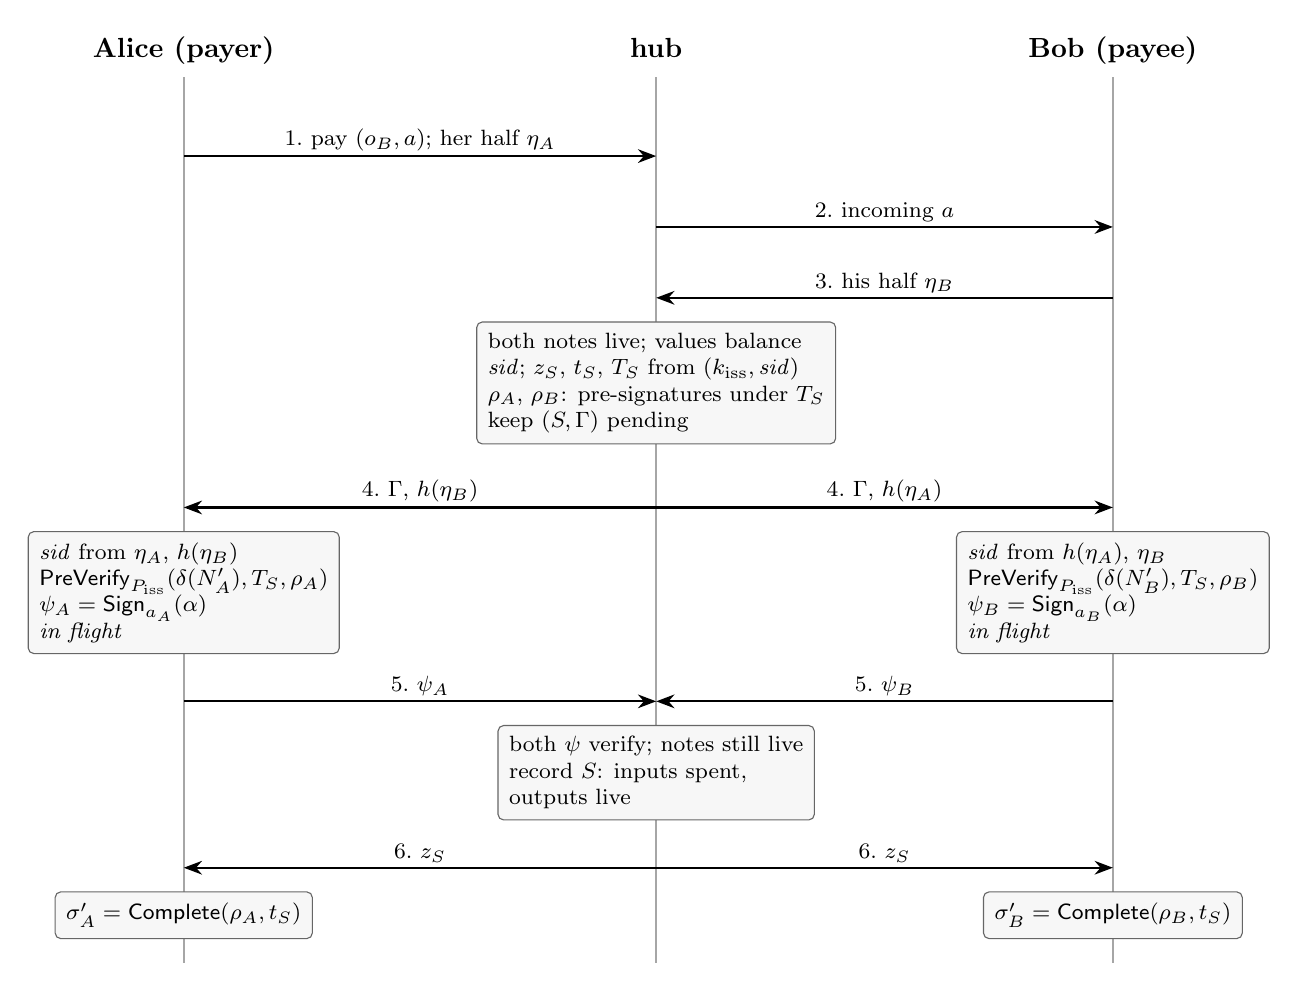
\begin{tikzpicture}[>=Stealth, font=\small,
  life/.style={draw=black!35, thick},
  box/.style={draw=black!60, fill=black!3, rounded corners=2pt, align=left, inner sep=4pt, font=\footnotesize},
  msg/.style={->, thick},
  lbl/.style={align=center, font=\footnotesize, inner sep=1.5pt}]
\coordinate (LA) at (2.4,0); \coordinate (LH) at (8.4,0); \coordinate (LB) at (14.2,0);
\node[font=\bfseries, anchor=base] at ($(LA)+(0,0.25)$) {Alice (payer)};
\node[font=\bfseries, anchor=base] at ($(LH)+(0,0.25)$) {hub};
\node[font=\bfseries, anchor=base] at ($(LB)+(0,0.25)$) {Bob (payee)};
\coordinate (y) at (0,-1.0);
\draw[msg] (LA|-y) -- node[lbl, above] {1.\ pay $(o_B, a)$; her half $\eta_A$} (LH|-y);
\coordinate (y) at ($(y)+(0,-0.9)$);
\draw[msg] (LH|-y) -- node[lbl, above] {2.\ incoming $a$} (LB|-y);
\coordinate (y) at ($(y)+(0,-0.9)$);
\draw[msg] (LB|-y) -- node[lbl, above] {3.\ his half $\eta_B$} (LH|-y);
\node[box, anchor=north] (b1) at ($(LH|-y)+(0,-0.3)$) {
  both notes live; values balance\\
  $\sid$; $z_S$, $t_S$, $T_S$ from $(\kiss, \sid)$\\
  $\rho_A$, $\rho_B$: pre-signatures under $T_S$\\
  keep $(S, \Gamma)$ pending};
\coordinate (y) at ($(b1.south)+(0,-0.8)$);
\draw[msg] (LH|-y) -- node[lbl, above] {4.\ $\Gamma$, $h(\eta_B)$} (LA|-y);
\draw[msg] (LH|-y) -- node[lbl, above] {4.\ $\Gamma$, $h(\eta_A)$} (LB|-y);
\node[box, anchor=north] (b2) at ($(LA|-y)+(0,-0.3)$) {
  $\sid$ from $\eta_A$, $h(\eta_B)$\\
  $\PVfy_{\Piss}(\delta(N'_A), T_S, \rho_A)$\\
  $\psi_A = \Sign_{a_A}(\alpha)$\\
  \emph{in flight}};
\node[box, anchor=north] (b3) at ($(LB|-y)+(0,-0.3)$) {
  $\sid$ from $h(\eta_A)$, $\eta_B$\\
  $\PVfy_{\Piss}(\delta(N'_B), T_S, \rho_B)$\\
  $\psi_B = \Sign_{a_B}(\alpha)$\\
  \emph{in flight}};
\coordinate (y) at ($(b2.south)+(0,-0.6)$);
\draw[msg] (LA|-y) -- node[lbl, above] {5.\ $\psi_A$} (LH|-y);
\draw[msg] (LB|-y) -- node[lbl, above] {5.\ $\psi_B$} (LH|-y);
\node[box, anchor=north] (b4) at ($(LH|-y)+(0,-0.3)$) {
  both $\psi$ verify; notes still live\\
  record $S$: inputs spent,\\
  outputs live};
\coordinate (y) at ($(b4.south)+(0,-0.6)$);
\draw[msg] (LH|-y) -- node[lbl, above] {6.\ $z_S$} (LA|-y);
\draw[msg] (LH|-y) -- node[lbl, above] {6.\ $z_S$} (LB|-y);
\node[box, anchor=north] (b5) at ($(LA|-y)+(0,-0.3)$) {$\sigma'_A = \Compl(\rho_A, t_S)$};
\node[box, anchor=north] (b6) at ($(LB|-y)+(0,-0.3)$) {$\sigma'_B = \Compl(\rho_B, t_S)$};
\coordinate (end) at ($(b5.south)+(0,-0.3)$);
\begin{scope}[on background layer]
\foreach \l in {LA,LH,LB} \draw[life] (\l) -- (\l|-end);
\end{scope}
\end{tikzpicture}
\caption{A live payment: a joint spend of both notes. Each party is in
flight from its signature (step 5) until it has $z_S$ (step 6). Either
can hand $z_S$ to the other.}
\label{fig:payment}
\end{figure}

The payment is complete for a party when it holds $z_S$: then its new
note is settled. Alice's receipt is $z_S$; Bob's acceptance is his
$\psi_B$, which the hub can show her. Either party holding $z_S$ can
hand it to the other, so neither depends on the hub to learn that the
other side completed.

\textbf{In flight.} From its signature until it holds $z_S$, a party
keeps its old note and $(S, \Gamma)$. It claims its old note with $S$
as a \emph{fallback} (\S\ref{sec:claim}): if the hub uses $S$ against the
claim, it must publish $z_S$, and the new note counts instead.

\subsection{Rules}\label{sec:rules}

\textbf{Rule 1 (the statement): a spend counts only with both owners'
signatures.} A cited spend is usable against a claim only if $\psi_1$
and $\psi_2$ both verify on $\alpha$ (\S\ref{sec:statement}). Without
this, the hub could take $\psi_A$ alone, cite $S$ against Alice, and
publish $z_S$ to a Bob who never signed, and so may not hold the grant:
she would be debited and no one paid. With it, $S$ counts against no one
until both have signed; and both signers hold the grant, so whichever
exit publishes $z_S$ settles both new notes.

\textbf{Rule 2 (the wallet): one pending signature per key.} A wallet
never signs a spend while another it signed is pending. Otherwise the
hub could complete two spends of one note: if Bob signed two incoming
payments, each would count against its payer, and his claim could
follow only one. The hub can't make a wallet break this rule. It means
one payment at a time per user, in either direction: Bob can't be paid
while his own payment is pending, nor be paid twice at once. An honest
hub tells a second payer \emph{busy, retry}.

\textbf{Rule 3 (the wallet): sign only spends of your current note.}
Each owner checks its half: its input is the note it holds, its output
the value it expects. So the invariant of one note is the owner's own,
whatever the hub does.

\textbf{Cancelling.} A party in flight asks the hub to cancel. If the
hub holds both signatures, it answers with $z_S$: the payment is done.
Otherwise it \emph{reissues} the party's note,
\[
  N^{*} = \big(\Ht{issue}(\texttt{"reissue"} \,\|\, \iota),\ o,\ v\big),
\]
the same owner and value under a fresh id, with $\sigma_{N^*}$; marks the old note
cancelled; and refuses $S$ from then on. The party now holds $N^*$ and
nothing in flight. If the hub completed $S$ anyway, $S$ would take the
old note, which no claim names any more: the hub pays the counterparty
from nothing. So a reissue needs no certificate: it is just a note.

\subsection{What atomicity means here}\label{sec:atomic}

Once both have signed, the hub may record $S$ or not.
\begin{itemize}[nosep]
\item Not recorded, or cancelled: the hub alone knows $t_S$; the new
  notes never settle, and the old ones (or their reissues) stand.
\item Recorded, $z_S$ given to either party: both are paid, since the
  other can be handed $z_S$.
\item Recorded, $z_S$ withheld from both: both are in flight, and
  neither exit can be reduced through $S$ without publishing $z_S$,
  which settles both new notes.
\end{itemize}
Version 0.4's atomicity was one-way: the chain enforced the payer's
side, and the payee was paid only once he held a settled note. Here
both sides are payers of a note, and both are protected the same way.

\textbf{Settling into a closed contract.} One gap remains, and version
0.4 has it too. Suppose the hub records $S$, withholds $z_S$, and Bob
exits first, naming $S$ as his fallback. The hub doesn't cite $S$
against him (it would raise what he is owed), so he is paid $v_B$.
Later the hub cites $S$ against Alice: she is debited $a$, and Bob's new
note settles under a key whose contract has closed, as credit. The hub
keeps $a$. The order is what matters: had Alice exited first, $S$ would
either have been cited, settling Bob's note while his contract was
open, or not, leaving both whole. So the rule for a halt is
\textbf{payers exit first}: a payee with an incoming payment in flight
waits for its payer's exit to pass \tx{correct} (or its window), as
long as its own close allows.
Both are online parties to the payment, so they can arrange it; a payer
who never exits is either the hub itself, whose payment Bob never
counted, or leaves her contract to default, where she loses more than
$a$. At stake, at most one payment per user, and only one the hub has
deliberately left pending.

\section{The contract}\label{sec:contract}

\textbf{Opening and the mint} are version 0.4's (\cite{grants04},
\S4.1): the mint $N_0 = (\Ht{issue}(\texttt{"mint"} \,\|\, \be{c}{4}),
\Oc, v_0)$ exists exactly when the funding transaction confirms, and
its evidence is the journal, which binds $v_0$. The mint is $\Oc$'s
first note; her first payment, in or out, takes it as her half's input.

\textbf{The journal}, the statement's public input:
\begin{align*}
  J &= \be{c}{4} \,\|\, D,\qquad
  D = \mathrm{SHA256}\big(\texttt{"lichen/grants/contract"} \,\|\,
  \xo{\Piss} \,\|\, \xo{\Oc} \,\|\, \be{u}{8} \,\|\, \be{v_0}{8} \,\|\,
  \kappa\big),\\
  \kappa &= \mathrm{SHA256}\big(\KQ \,\|\, \Kb \,\|\, \Acorr \,\|\, \AU\big).
\end{align*}
Only the issuer's key changes from version 0.4: a secp256k1 key in
place of BLS's $I$.

\textbf{The dispute graph} is version 0.4's unchanged
(Figure~\ref{fig:graph}): \tx{request}, \tx{correct}, \tx{ack},
\tx{assert}, \tx{challenge\_assert}, with the terminals \tx{fold},
\tx{default}, \tx{request\_timeout}, \tx{accept}, \tx{ack\_timeout},
\tx{success}, \tx{wrongly\_challenged\_$k$} and \tx{failure}; payouts in
bits, each bit output spent by re-presenting the one-time signature on
the amount, with an equivocation leaf for the other party
(\cite{grants04}, \S4.3--4.4). Only the lengths change: $Q$ is 95 bytes
and $U$ 32 (\S\ref{sec:costs}).

\begin{figure}[!tbp]
\centering
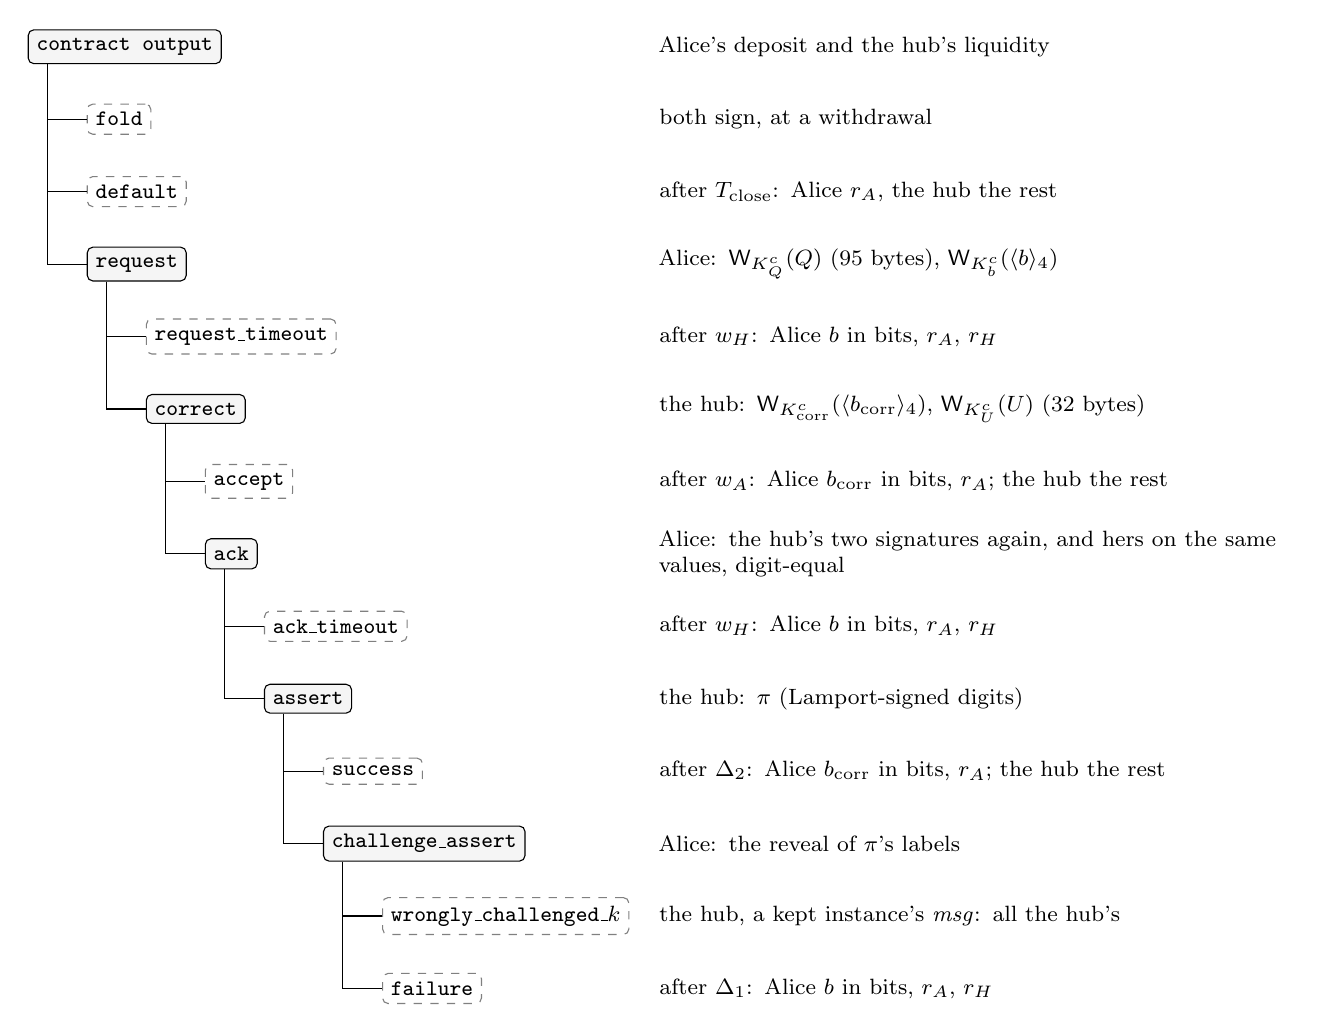
\begin{tikzpicture}[font=\footnotesize,
  link/.style={draw, rounded corners=2pt, inner sep=3pt, fill=black!4, font=\footnotesize\ttfamily, anchor=west},
  term/.style={draw=black!50, dashed, rounded corners=2pt, inner sep=3pt, font=\footnotesize\ttfamily, anchor=west},
  ann/.style={anchor=west, align=left, text width=7.9cm, font=\footnotesize}]
\def\dx{0.75}\def\dy{0.92}\def\ax{7.9}
\node[link] (c)  at (0*\dx, 0)       {contract output};
\node[term] (fo) at (1*\dx, -1*\dy)  {fold};
\node[term] (de) at (1*\dx, -2*\dy)  {default};
\node[link] (rq) at (1*\dx, -3*\dy)  {request};
\node[term] (rt) at (2*\dx, -4*\dy)  {request\_timeout};
\node[link] (co) at (2*\dx, -5*\dy)  {correct};
\node[term] (ac) at (3*\dx, -6*\dy)  {accept};
\node[link] (ak) at (3*\dx, -7*\dy)  {ack};
\node[term] (at) at (4*\dx, -8*\dy)  {ack\_timeout};
\node[link] (as) at (4*\dx, -9*\dy)  {assert};
\node[term] (su) at (5*\dx, -10*\dy) {success};
\node[link] (ch) at (5*\dx, -11*\dy) {challenge\_assert};
\node[term] (wc) at (6*\dx, -12*\dy) {wrongly\_challenged\_$k$};
\node[term] (fa) at (6*\dx, -13*\dy) {failure};
\foreach \p/\q in {c/fo,c/de,c/rq,rq/rt,rq/co,co/ac,co/ak,ak/at,ak/as,as/su,as/ch,ch/wc,ch/fa}
  \draw ($(\p.south west)+(0.25,0)$) |- (\q.west);
\node[ann] at (\ax, 0)         {Alice's deposit and the hub's liquidity};
\node[ann] at (\ax, -1*\dy)    {both sign, at a withdrawal};
\node[ann] at (\ax, -2*\dy)    {after $\Tc$: Alice $r_A$, the hub the rest};
\node[ann] at (\ax, -3*\dy)    {Alice: $\Wots_{\KQ}(Q)$ (95 bytes), $\Wots_{\Kb}(\be{b}{4})$};
\node[ann] at (\ax, -4*\dy)    {after $w_H$: Alice $b$ in bits, $r_A$, $r_H$};
\node[ann] at (\ax, -5*\dy)    {the hub: $\Wots_{\Kcorr}(\be{\bcorr}{4})$, $\Wots_{\KU}(U)$ (32 bytes)};
\node[ann] at (\ax, -6*\dy)    {after $w_A$: Alice $\bcorr$ in bits, $r_A$; the hub the rest};
\node[ann] at (\ax, -7*\dy)    {Alice: the hub's two signatures again, and hers on the same values, digit-equal};
\node[ann] at (\ax, -8*\dy)    {after $w_H$: Alice $b$ in bits, $r_A$, $r_H$};
\node[ann] at (\ax, -9*\dy)    {the hub: $\pi$ (Lamport-signed digits)};
\node[ann] at (\ax, -10*\dy)   {after $\Delta_2$: Alice $\bcorr$ in bits, $r_A$; the hub the rest};
\node[ann] at (\ax, -11*\dy)   {Alice: the reveal of $\pi$'s labels};
\node[ann] at (\ax, -12*\dy)   {the hub, a kept instance's \textit{msg}: all the hub's};
\node[ann] at (\ax, -13*\dy)   {after $\Delta_1$: Alice $b$ in bits, $r_A$, $r_H$};
\end{tikzpicture}
\caption{A contract's graph, as in version 0.4: solid boxes carry the
value on, dashed ones are terminals.}
\label{fig:graph}
\end{figure}

\textbf{Withdrawal.} Alice hands the hub a claim (\S\ref{sec:claim})
signed with $a_c$. The hub takes it if its book shows the note live: it
marks the note taken, and both sign the fold, which pays her $u\,b$ and
$r_A$. What the note held beyond $u\,b$ the hub issues to her wallet's
key with no contract, as credit.

\section{The exit}\label{sec:exit}

\subsection{The claim}\label{sec:claim}

\begin{definition}
A \emph{claim} on contract $c$ is $(b;\ N;\ p)$: her one note $N$ (the
mint, by a flag $\mu$, or a settled note of $\Oc$ with $\sigma_N$); and
at most one fallback, the first 8 bytes $p$ of the id of the spend she
has in flight, if any; with $b \le \lfloor v/u \rfloor$, $v$ the note's
value ($v_0$ for the mint).
\end{definition}

\textbf{The posted claim} $Q$, exactly $L_Q = 95$ bytes:
\[
  Q = \be{\mu + 2\phi}{1} \,\|\, \pre{\mathit{id}}{16} \,\|\,
  \be{v}{6} \,\|\, \sigma_N^{(64)} \,\|\, p^{(8)},
\]
$\phi$ whether a fallback is present; for the mint, zeros in place of
the note, and for no fallback, zeros in place of $p$. The mint, the
contract and $v_0$ come from the journal; $b$ is signed under its own
key, as in version 0.4.

A claim covers her whole balance, always: there is no subset to choose,
and no capacity to exceed. What an offline receiver had protected in
version 0.4 (at most four notes) has no counterpart, because there is
no offline receiver (but see \S\ref{sec:deferred}).

\subsection{The hub's correction and her answer}\label{sec:correct}

As in version 0.4 (\cite{grants04}, \S5.2--5.3). When \tx{request}
appears, the hub maps the note (or mint) and the fallback to its book;
computes $x = \owed(\cdot)$ (Algorithm~1) with the statement's own
function; takes the claim into its book at $x$; and if $x < b$ posts
\tx{correct} with $\bcorr = x$ and the seeds $U$ of the (at most two)
spends it cites. Alice reads $U$: if it opens her spend in flight, she
completes her new note and hands $z_S$ to the counterparty. Then she
accepts, or contests by \tx{ack}: her countersignatures on $\bcorr$ and
$U$, digit-equal to the hub's.

\subsection{The hub's statement}\label{sec:statement}

\emph{The claim Alice signed is owed at most the $\bcorr$ she
countersigned.}

\textbf{Private input}: her four one-time public keys and the four
signatures under them, from \tx{request} and \tx{ack}: $\Wots_{\KQ}(Q)$,
$\Wots_{\Kb}(\be{b}{4})$, $\Wots_{\Acorr}(\be{\bcorr}{4})$ and
$\Wots_{\AU}(U)$; $v_0$; and the cited spends $X_1, \dots, X_q$, $q \le
2$, each
\[
  X = \big(\eta_X,\ o'_X,\ h'_X,\ T_X^{(33)},\ \rho_{X,1}, \rho_{X,2},\
  \psi_{X,1}, \psi_{X,2}\big):
\]
her half $\eta_X$ (owner $\Oc$), the other owner and its half's digest,
the grant's point and pre-signatures, and both owners' signatures. From
these the statement recomputes $\sid_X$ (ordering the two owners),
$C_X$ and $\alpha_X$ as in \S\ref{sec:grant}. The other half stays a
digest: the statement never learns the counterparty's balance.

\textbf{Checks}, in order (any failure rejects; no proof):
\begin{enumerate}[nosep]
\item The keys hash to $\kappa$, and $\be{c}{4} \,\|\, D = J$.
\item The four one-time signatures verify; their digits give $Q$, $b$,
  $\bcorr$, $U$.
\item $\owed(Q, b, \Oc, u, v_0, (X_q), U) \le \bcorr$ (Algorithm~1).
\end{enumerate}
\textbf{Output}: $J$.

\begin{algobox}{Algorithm 1: $\owed(Q, b, O, u, v_0, (X_q), U)$, in units}
\textbf{Malformed: return 0} if $Q$ doesn't parse; or $\mu = 0$ and not
$\Vfy_{\Piss}(\delta(N), \sigma_N)$, $N = (\iota, O, v)$; or $b > \lfloor
v/u \rfloor$. (For the mint, $\iota = \pre{\mathit{id}_0}{16}$ and $v =
v_0$.)\\[3pt]
\textbf{Usable.} $X$ is usable iff (a) $\Vfy_{o_i}(\alpha_X,
\psi_{X,i})$ for both owners, one of them $O$, whose half is
$\eta_X$; (b) some nonzero word $z$ of $U$ has
$t\,G = T_X$, $t$ its scalar. $X$ \emph{takes} $\iota$ if it is usable
and its half's input is $\iota$.\\[3pt]
\textbf{1.} If no $X$ takes $\iota$: \textbf{return} $\min(b, \lfloor
v/u \rfloor)$.\\
\textbf{2.} If some $X$ that takes $\iota$ has $\pre{\sid_X}{8} = p$:
let $\iota' = \pre{\Ht{out}(\sid_X, O)}{16}$ and $v'$ her half's output.
If no $Y$ takes $\iota'$: \textbf{return} $\min(b, \lfloor v'/u
\rfloor)$; else \textbf{return} 0.\\
\textbf{3.} \textbf{Return} 0.
\end{algobox}

Case 1: her note is unspent. Case 2: it went into her spend in flight,
which the hub cites, so her new note counts, unless she spent that too.
Case 3: it went into a spend she didn't name, or into her new note's
own spend: a stale claim, owed nothing. Version 0.4's fixed point over
sets, its revivals keyed by prefix and its double-count argument, all
drop out: there is one candidate, and one revival at most.

\textbf{Faked evidence only hurts the hub.} As before: evidence only
lowers what she is owed, and evidence failing a check kills nothing.

\subsection{How much evidence a claim can need}\label{sec:volume}

\begin{proposition}\label{prop:volume}
For any claim and any set of usable spends, at most two of them affect
Algorithm~1: one taking $\iota$ and, if it is the fallback, one taking
$\iota'$. So $U$'s two seeds suffice.
\end{proposition}

That is the whole of version 0.4's capacity argument (\cite{grants04},
Proposition~1).

\subsection{What each side gets}\label{sec:who}

\begin{proposition}[the honest user]\label{prop:user}
Let Alice claim the note she holds, naming as fallback the spend she
has in flight, if any, and let her one-time keys sign only in
\tx{request} and \tx{ack}. Then she is paid at least $\min(b, \lfloor
x/u \rfloor)$, where $x$ is her note's value, or her new note's if the
hub cites her spend in flight; and in that case $U$ holds its seed, so
the payment completes for both parties.
\end{proposition}

\begin{proposition}[the hub]\label{prop:hub}
If every spend the hub records satisfies the statement's checks, and
the hub moves within $w_H$, then for any claim it pays at most the value
of $\Oc$'s live note in its book, at most $b$; a malformed or stale claim
gets 0.
\end{proposition}

The arguments are version 0.4's, shortened: a usable spend carries her
own signature on a grant she checked; the one she names is cited only
with its seed; and the hub, holding every recorded spend with both
signatures, can always cite the one that took a stale note.

\textbf{Who must be online.} For a payment, both parties and the hub.
For an exit, as in version 0.4: the hub for \tx{correct} and
\tx{assert}; Alice to contest within $w_A$, with keys.

\section{Option: deferred receipt}\label{sec:deferred}

The live design asks the payee to be online when paid. A mailbox can
relax that, at a price. Alice signs first; the hub keeps the spend in
Bob's mailbox; Bob signs when he next connects; then the hub releases
$z_S$ to both. Rule 1 already makes this safe in one direction: until
Bob signs, $S$ counts against no one, so Alice can't be debited for a
payment Bob never accepted. What has to be added:

\begin{enumerate}[nosep]
\item \textbf{The hub forms the payee's half.} Bob's half takes his
  current note, which Alice must not see; so the hub writes $\eta_B$,
  with a blinding of its own, and Bob checks it when he signs. A half
  he finds wrong, he refuses.
\item \textbf{One payment per payee in the mailbox.} A second payment to
  Bob would take the note the first one produces, which doesn't exist
  until he signs. So the hub queues later payers without forming their
  spends, and they sign only when their turn comes: they must be online
  then, or the queue skips them.
\item \textbf{The payer is in flight while the payee is away.} Alice's
  note is locked for as long as Bob stays offline, and by Rule 2 she
  can make no other payment. Her wallet cancels after a timeout
  (\S\ref{sec:rules}), and the cancel races Bob's signature: the hub
  serializes them, answering her with $z_S$ if his arrived first.
\item \textbf{Late signatures.} Bob may sign a spend Alice already
  cancelled. The hub refuses it, so Bob is now in flight on a spend that
  will never complete, and needs a reissue of his own. Every pending
  spend can strand both of its parties, not one.
\item \textbf{Settling into a closed contract} (\S\ref{sec:atomic})
  becomes likelier: the window in which a payment is pending is now as
  long as the payee's absence, not a round trip.
\end{enumerate}

None of this reintroduces several notes per key, so the exit, the
statement and Algorithm~1 are unchanged: the cost is all in the
payment protocol and the wallet's timeouts. The alternative, letting an
offline payee accumulate separate notes and merge later, is version
0.4.

\section{Costs}\label{sec:costs}

Link sizes scaled from version 0.4's graph as measured on regtest
(\tx{request} 8,891 vB with 578 stack items; \tx{correct} 3,611 with
284; \tx{ack} 8,025 with 566), in proportion to stack items. Statement
cycles from measured parts: a BIP340 verification is about 260k cycles
in the chain guest; SHA-256 compressions about 490 each. Nothing in
this version is built.

\begin{center}
\begin{tabularx}{\linewidth}{lL}
\toprule
Item & Cost (est.) \\
\midrule
\tx{request} & $Q$ (95 bytes) and $b$: $2(190 + 4) + 2(8 + 2) + 2 = 410$ items, about 6.3 kvB \\
\tx{correct} & $\bcorr$ and $U$ (32 bytes): $2(8 + 2) + 2(64 + 3) + 2 = 156$ items, about 2.0 kvB \\
\tx{ack} & both parties' signatures on both: 310 items, about 4.4 kvB \\
statement & her one-time signatures, about 280 chains, some 2,100 compressions: 1.0M; the note's signature and up to four $\psi$: 5 BIP340 checks, 1.3M; up to two $t\,G$: about 0.3M. About 2.6M cycles, 3 segments, against version 0.4's 29M; proving in minutes on a laptop \\
payment & about two round trips for each party; each checks one pre-signature and makes one BIP340 signature \\
\bottomrule
\end{tabularx}
\end{center}

Every on-chain witness stays well inside Bitcoin's 1,000 stack items;
the largest, \tx{request}, uses 410.

\section{What one note wins, and what it costs}\label{sec:compare}

\begin{center}
\begin{tabularx}{\linewidth}{lLL}
\toprule
& Version 0.4: many notes & Version 0.5: one note \\
\midrule
receiving & offline, by mailbox & online, signing (deferred: \S\ref{sec:deferred}) \\
notes per key & any; an exit protects 4 & exactly 1, all of it protected \\
merges & needed, and need the hub & none \\
a halting hub keeps & every note beyond each claim's 4 & nothing \\
claim $Q$ & 137 bytes; $\mu + n + f \le 4$ & 95 bytes; a note and $\le 1$ fallback \\
unlocks $U$ & 4 seeds, 64 bytes & 2 seeds, 32 bytes \\
\tx{request}, \tx{correct}, \tx{ack} & 8.9, 3.6, 8.0 kvB (measured) & 6.3, 2.0, 4.4 kvB (scaled) \\
Algorithm~1 & fixed point over a set; revivals by prefix & three cases \\
capacity proof & $|K| \le \mu + n + f$, each cited spend kills one entry & two spends, by inspection \\
note signatures & BLS, aggregated; encrypted under $T$ & BIP340; adaptor pre-signatures \\
statement & about 29M cycles (a pairing) & about 2.6M (no pairing) \\
concurrency & up to 3 spends in flight, as fallbacks & one pending signature per key \\
atomicity & one-way: the payer's side & both sides, the same way \\
a cancelled payment & stays in flight & reissued note \\
the counterparty learns & the payee nothing of her change & the amount only (halves) \\
\bottomrule
\end{tabularx}
\end{center}

\textbf{Simpler.} The exit loses its only intricate part, Algorithm~1's
fixed point, and the argument that four seeds suffice. The wallet loses
its merge policy and its choice of which notes to claim. The hub's
statement loses BLS entirely, and with it the measured cost that made
proving the open question of version 0.4: 29M cycles, half an hour on a
laptop, becomes about 2.6M, a few minutes. And the instability of
version 0.4, a hub that can estimate what it would keep by halting,
has nothing to act on.

\textbf{What it costs.} Payees must be online, and each user makes one
payment at a time. These are Lightning's terms for a payee, without
channels or routes, and they suit a wallet that is open when it is
used. The deferred receipt of \S\ref{sec:deferred} buys back some
offline receipt, at the price of timeouts and cancellations in the
payment protocol, but not in the exit.

\textbf{The private variant.} One note per key needs arbitrary values,
so it doesn't combine with fixed-denomination ecash, where a balance
takes as many notes as its value has set bits. A private form would
need hidden amounts: keyed-verification credentials with amount
attributes, as in WabiSabi, whose verification key the journal would
have to commit to.

\section{Open questions}\label{sec:open}

\begin{itemize}[nosep]
\item \textbf{Settling into a closed contract} (\S\ref{sec:atomic}),
  here and in version 0.4: is \emph{payers exit first} enough, or can
  the statement bind a spend's use to the payee's contract being open?
\item \textbf{A keyless contest}, as in version 0.4: \tx{ack} needs her
  keys within $w_A$.
\item \textbf{Latency and liveness of a payment}: two round trips with
  both parties online. A payee's wallet must answer within seconds;
  how does a phone do it in the background?
\item \textbf{Fees.} A fee is naturally a third half, the hub's own
  note; that breaks the two-owner shape of a spend, or the fee is
  folded into the payer's half.
\item \textbf{Restoring a wallet} needs its current note, which the hub
  can resend; a restore from an old backup claims a stale note, owed 0
  (Algorithm~1, case 3), unless the hub cooperates.
\item \textbf{Measurement}: the statement's cycles and the links' sizes
  are estimates scaled from version 0.4's measurements.
\end{itemize}

\begin{thebibliography}{9}
\bibitem{lichen} waxwing, \emph{Lichen}, version 0.5, 2026.
\bibitem{grants04} waxwing, \emph{The grants L2: the countersigned exit,
  with BLS notes}, version 0.4, November 2026.
\bibitem{bip340} P.~Wuille, J.~Nick, T.~Ruffing, \emph{BIP 340: Schnorr
  signatures for secp256k1}, 2020.
\bibitem{poelstra} A.~Poelstra, \emph{Scriptless scripts}, 2017.
\bibitem{aumayr} L.~Aumayr, O.~Ersoy, A.~Erwig, S.~Faust,
  K.~Hostáková, M.~Maffei, P.~Moreno-Sanchez, S.~Riahi,
  \emph{Generalized channels from limited blockchain scripts and
  adaptor signatures}, ASIACRYPT 2021.
\end{thebibliography}

\end{document}
